\chapter{Dataset}
\label{sec:dataset}


% use [] to set name for ToC
\section[Informazioni introduttive]{Informazioni introduttive} % ok with fontsize=12pt
I dati utilizzati sono divisibili in tre diverse categorie:
\begin{itemize}
\item  Dati dei circuiti, dei piloti e delle scuderie e relative prestazioni in tutte le gare;
\item  Dati utlizzati per quantificare il valore tecnico di ciascun pilota;
\item  Dati riguardanti gli investimenti fatti dalle scuderie nel 2020.
\end{itemize}
Il software è stato realizzato per poter essere aggiornato con le prestazioni dei piloti e delle scuderie negli anni successivi.\\
A scopo di esempio e per testare le funzionalità dell'applicazione sono stati utilizzati i dati riguardanti tutte le stagioni fino alla fine del campionato di F1 del 2020. Tali dati sono stati estratti al seguente indirizzo: \href{http://ergast.com/mrd/db/}{http://ergast.com/mrd/db/}. Allo script sql, rilasciato con licenza Attribution-NonCommercial-ShareAlike 3.0 Unported Licence, è poi necessario aggiungere uno script sql che comprende una tabella per assegnare i punteggi ad ogni pilota ed una tabella che riporta gli importi spese dalle scuderie.\\
Nella directory "db" è possibile trovare un file in formato sql che contiene al suo interno sia i dati delle prestazioni sia i dati riguardanti il punteggio dei piloti e le spese dei vari team; è inoltre disponibile anche il solo esempio dei punteggi e delle spese ed è anche disponibile un altro file utile se si ha già un database chiamato "F1"

\begin{figure}[h]
\centering
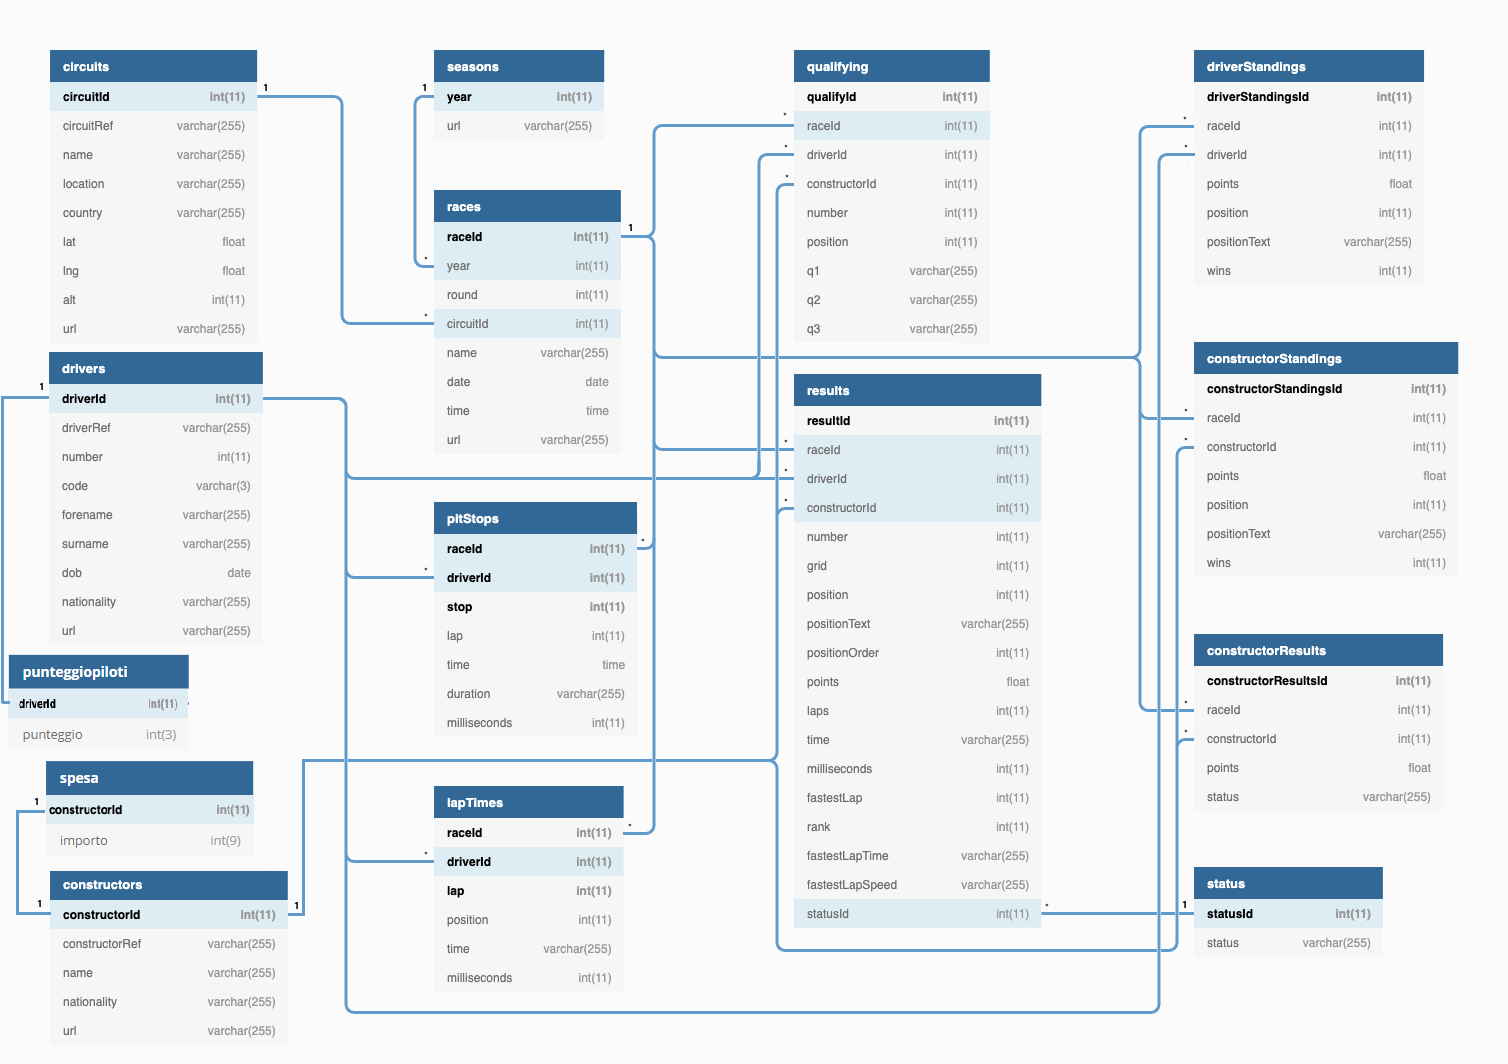
\includegraphics[width=1\linewidth]{images/Diagramma ER.png}
\caption{Diagramma ER}
\label{fig:Diagramma ER}
\end{figure}

\section[Descrizione delle tabelle]{Descrizione delle tabelle}
\subsection{tabella circuits}% ok with fontsize=12pt
\begin{enumerate}
    \item\textbf{ circuitid}: codice identificativo del circuito;
    \item \textbf{circuitRef}: stringa identificativa per il circuito;
    \item \textbf{name}: nome del circuito;
    \item \textbf{location}: città in cui si trova il circuito;
    \item \textbf{country}: Paese in cui si trova il circuito;
    \item \textbf{lat}: latitudine del punto in cui si trova il circuito;
    \item \textbf{lng}: longitudine del punto in cui si trova il circuito;
    \item \textbf{alt};
    \item \textbf{url}: link wikipedia del circuito;
\end{enumerate}
\subsection{tabella drivers}% ok with fontsize=12pt
\begin{enumerate}
    \item \textbf{driversid}: codice identificativo del pilota;
    \item \textbf{driverRef}: stringa identificativa per il pilota (generalmente uguale al surname);
    \item \textbf{number}: numero utilizzato dal pilota;
    \item \textbf{code}: stringa di 3 caratteri per identificare il pilota;
    \item \textbf{forename}: nome del pilota;
    \item \textbf{surname}: cognome del pilota;
    \item \textbf{dob}:data di nascita del pilota;
    \item \textbf{nationality}: Paese del pilota;
    \item \textbf{url}: link wikipedia del pilota;
\end{enumerate}
\subsection{tabella constructors}% ok with fontsize=12pt
\begin{enumerate}
    \item \textbf{constructorId}: codice identificativo della scuderia;
    \item \textbf{constructorRef}: stringa identificativa per la scuderia (generalmente uguale al name);
    \item \textbf{nome}: nome della scuderia;
 \textbf{nationality}: Paese della scuderia;
    \item \textbf{url}: link wikipedia della scuderia;
\end{enumerate}
\subsection{tabella races}% ok with fontsize=12pt
\begin{enumerate}
    \item \textbf{raceid}: codice identificativo della gara;
    \item \textbf{year}: anno di svolgimento della gara;
    \item \textbf{round}: numero progressivo annuale;
    \item \textbf{circuitid}: codice identificativo del circuito;
    \item \textbf{name}: nome che viene dato alla gara;
    \item \textbf{data}: data in cui si svolge la gara;
    \item \textbf{time}: orario in cui si svolge la gara;
    \item \textbf{url}: link wikipedia della gara;
\end{enumerate}
\subsection{tabella pitStops}% ok with fontsize=12pt
\begin{enumerate}
    \item \textbf{raceid}: codice identificativo della gara;
    \item \textbf{driverid}: codice identificativo;
    \item \textbf{stop}: numero progressivo di stop per ogni pilota per ogni gara;
    \item \textbf{lap}: giro in cui è stato effettuato il pitstop;
    \item \textbf{time}: ora in cui è stato effettuato il pitstop;
    \item \textbf{duration}: durata del pitstop;
    \item \textbf{milliseconds}: durata del pitsop in millisecondi;
\end{enumerate}
\subsection{tabella lapTimes}% ok with fontsize=12pt
\begin{enumerate}
    \item \textbf{raceid}: codice identificativo della gara;
    \item \textbf{driverid}: codice identificativo del pilota;
    \item \textbf{lap}: giro in cui è stato effettuato il pitstop;
    \item \textbf{position}: posizione in cui si trova il pilota all'inizio del giro;
    \item \textbf{time}: durata del giro;
    \item \textbf{milliseconds}: durata del pitsop in millisecondi;
\end{enumerate}
\subsection{tabella qualifying}% ok with fontsize=12pt
\begin{enumerate}
    \item qualifyid: codice identificativo della qualifica, diverso per ogni gara e per ogni pilota;
    \item \textbf{raceid}: codice identificativo della gara;
    \item \textbf{driverid}: codice identificativo del pilota;
    \item \textbf{constructorid}: codice identificativo della scuderia;
    \item \textbf{number}: numero del pilota;
    \item \textbf{position}: posizione guadagnata dal pilota in griglia di partenza;
    \item \textbf{q1}: durata del miglior giro in q1;
    \item \textbf{q2}: durata del miglior giro in q2;
    \item \textbf{q3}: durata del miglior giro in q3;
\end{enumerate}
\subsection{tabella results}% ok with fontsize=12pt
\begin{enumerate}
    \item \textbf{resultid}: codice identificativo del risultato di una gara;
    \item \textbf{raceid}: codice identificativo della gara;
    \item \textbf{driverid}: codice identificativo del pilota;
    \item \textbf{constructorid}: codice identificativo della scuderia;
    \item \textbf{number}: numero del pilota;
    \item \textbf{grid}: posizione iniziale del pilota;
    \item \textbf{position}: posizione finale del pilota (null per piloti che si sono ritirati durante la gara);
    \item \textbf{positionText}: viene riportato sotto forma di stringa la posizione o il motivo di ritiro;
    \item \textbf{positionOrder}: posizione finale del pilota;
    \item \textbf{points}: punti guadagnati in gara;
    \item \textbf{laps}: numero di giri compiuti;
    \item \textbf{time}: durata della gara;
    \item \textbf{milliseconds}: durata della gara in millisecondi;
    \item \textbf{fastestLap}: indicazione del giro in cui è stato fatto il miglior tempo;
    \item \textbf{rank}: posizione rispetto agli altri piloti per quanto riguarda i giri veloci;
    \item \textbf{fastestLapTime}: durata in millisecondi del miglior giro del pilota;
    \item \textbf{fastestLapSpeed}: velocità media di percorrenza del giro veloce;
    \item \textbf{statusId} : numero che corrisponde allo status del pilota ( nella tabella status viene indicato a cosa corrisponde ogni numero);
\end{enumerate}
\subsection{tabella driverStandings}% ok with fontsize=12pt
\begin{enumerate}
    \item \textbf{driverStandingsid}: codice identificativo del risultato del pilota in una gara;
    \item \textbf{raceid}: codice identificativo della gara;
    \item \textbf{driverid}: codice identificativo del pilota;
    \item \textbf{points}: punti guadagnati in gara;
   \item \textbf{position}: posizione finale del pilota (null per piloti che si sono ritirati durante la gara);
    \item \textbf{positionText}: viene riportato sotto forma di stringa la posizione o il motivo di ritiro;
    \item \textbf{wins}: valore binario per indicare la vittoria o no del pilota;
\end{enumerate}
\subsection{tabella constructorStandings}% ok with fontsize=12pt
\begin{enumerate}
    \item \textbf{constructorStandingsid}: codice identificativo del risultato della scuderia in una gara;
    \item \textbf{raceid}: codice identificativo della gara;
    \item \textbf{constructorid}: codice identificativo della scuderia;
    \item \textbf{points}: punti guadagnati in gara;
   \item \textbf{position}: posizione finale della scuderia;
    \item \textbf{positionText}: viene riportato sotto forma di stringa la posizione o il motivo di ritiro;
    \item \textbf{wins}: valore binario per indicare la vittoria o no della scuderia;
\end{enumerate}
\subsection{tabella constructorResults}% ok with fontsize=12pt
\begin{enumerate}
    \item \textbf{constructorResultsid}: codice identificativo del risultato della scuderia in una gara;
    \item \textbf{raceid}: codice identificativo della gara;
    \item \textbf{constructorid}: codice identificativo della scuderia;
    \item \textbf{points}: punti guadagnati in gara;
    \item \textbf{status}: variabile per indicare il motivo di ritiro della scuderia;
\end{enumerate}
